\documentclass{Vorlage}
%\usepackage[ngerman]{babel}
\usepackage{amsfonts}
\usepackage{graphicx}
\usepackage{url}
\usepackage{amsmath}
\usepackage{adjustbox}
\usepackage{color}
\usepackage{multirow}
\usepackage{bm}
%\usepackage[utf8]{inputenc}
%\bibliographystyle{apalike}
\setlength{\parindent}{0pt}

\pagestyle{fancy}
\renewcommand*\sectionmark[1]{\markboth{\MakeUppercase{#1}}{}}
\begin{document}

\newgeometry{top=2.5cm,bottom=2.0cm,left=2.5cm,right=2.5cm} % Befehl wird nur benötigt, falls Änderungen an den Seitenrändern in der Datei "Vorlage.cls" vorgenommen werden.

\begin{titlepage}

\begin{figure}
 \begin{center}
 
\includegraphics[scale=0.8]{Pictures/logo3}
 \end{center}
\end{figure}
\vspace*{3cm}




\titel{Kleinräumige Extrapolation von Umfragedaten}{}

\vspace{1cm}

\begin{tabular}{p{3.5cm}|p{0.1cm} p{10cm}l}
\textsc{Namen:} & & \textsc{Alexander Lange, Kai Husmann}\\
\textsc{Matr. Nr.:} & & \textsc{21426614}\\
\textsc{Studiengang:} & & \textsc{Angewandte Statistik}\\
\textsc{Mail:} & & \textsc{Alexander.lange$ @ $uni-goettingen.de}\\
\textsc{Kurs:} & & \textsc{Statistisches Praktikum}\\
\textsc{Kursleiter:} & & \textsc{Prof.Dr. Thomas Kneib}\\
\textsc{Lehrstuhl:} & & \textsc{Statistik}\\
\textsc{Fakultät:} & & \textsc{Wirtschaftswissenschaften}\\
\textsc{Date:} & & \textsc{\today}\\
\end{tabular}
\end{titlepage}

\restoregeometry

\pagenumbering{Roman} % \pagenumbering{roman} = Kleinschreibung: II -> ii.

\pagestyle{plain}

\tableofcontents % Inhaltsverzeichnis.

\newpage % Neue Seite.

\listoffigures % Abbildungsverzeichnis.

\listoftables % Tabellenverzeichnis.

\newpage

\pagenumbering{arabic} % Ab hier folgt die arabische Seitennummerierung.

%\renewcommand{\thesection}{\arabic{section}} % Römische Nummerierung der Kapitelüberschriften.

%============================================ Instroduction ========================================================%
\pagestyle{fancy}

\section{Einleitung}

\newpage

%=================================================== Main Part  ====================================================%
\section{Daten}
\subsection{Deskriptive Statistik}

\begin{table}[h]
\centering
\adjustbox{max height=\dimexpr\textheight-5.5cm\relax,
           max width=\textwidth}{
\begin{tabular}{l|c|c}
\multicolumn{2}{l}{Anzahl Beobachtungen Stichprobe: 3.143}     \\ \hline \hline
\textbf{Variable} & \textbf{Anzahl Klassen} & \textbf{Modellierung} \\ \hline
\textcolor{blue}{Bewertung Wohngegend} &  \textcolor{blue}{6} & \textcolor{blue}{Geordnet Kategorial} \\ \hline
\textcolor{blue}{Meinung Stuttgart 21} &  \textcolor{blue}{6} & \textcolor{blue}{Geordnet Kategorial} \\ \hline
Personenanzahl im Haushalt & 5 & Nicht Parametrisch \\ \hline
\textcolor{red}{Monatliches Netto Haushaltseinkommen} & \textcolor{red}{6} & \textcolor{red}{Nicht Parametrisch} \\ \hline
Altersklasse Befragter & 6 & Nicht Parametrisch \\ \hline
Geschlecht & 2 & Parametrisch\\ \hline
Familienstand & 4 & Parametrisch \\ \hline
Nationalität & 2 & Parametrisch \\ \hline
Stadtbezirk & 23 & Diskret Räumlich \\ \hline 
Stadtteil &  142 & Diskret Räumlich \\ \hline 
Gauß-Krüger & & Stetig Räumlich  \\ \hline \hline
\end{tabular}
}
\end{table}



\subsection{Räumliche Effekte}



\section{Methodik}

\subsection{Modell}

\subsection{Modellwahl}

\subsection{Evaluierung}

\section{Ergebnisse}



%\clearpage
%============================================== Conlcusion =========================================================%

\section{Ergebnisse}

\clearpage


%============================================ References ===========================================================%
\addcontentsline{toc}{section}{\numberline{}References}
\bibliographystyle{apalike}
\bibliography{} 

%\section{References}
%\renewcommand{\section}[2]{}
%\addcontentsline{toc}{section}{References}
%\renewcommand{\bibname}{4 References}
%\phantomsection
%\addcontentsline{toc}{section}{References}




\clearpage

%============================================== Appendix ============================================================%
%\appendix
%\pagestyle{Myheadings}
%\chead{APPENDIX}
%\pagestyle{}
%\section{$A^{-1}$ Appendix}
%\setcounter{secnumdepth}{0}



\begin{appendix}
\section*{Appendix}
\addcontentsline{toc}{section}{\numberline{}Appendix}
\begin{figure}[h]
 \begin{center}
 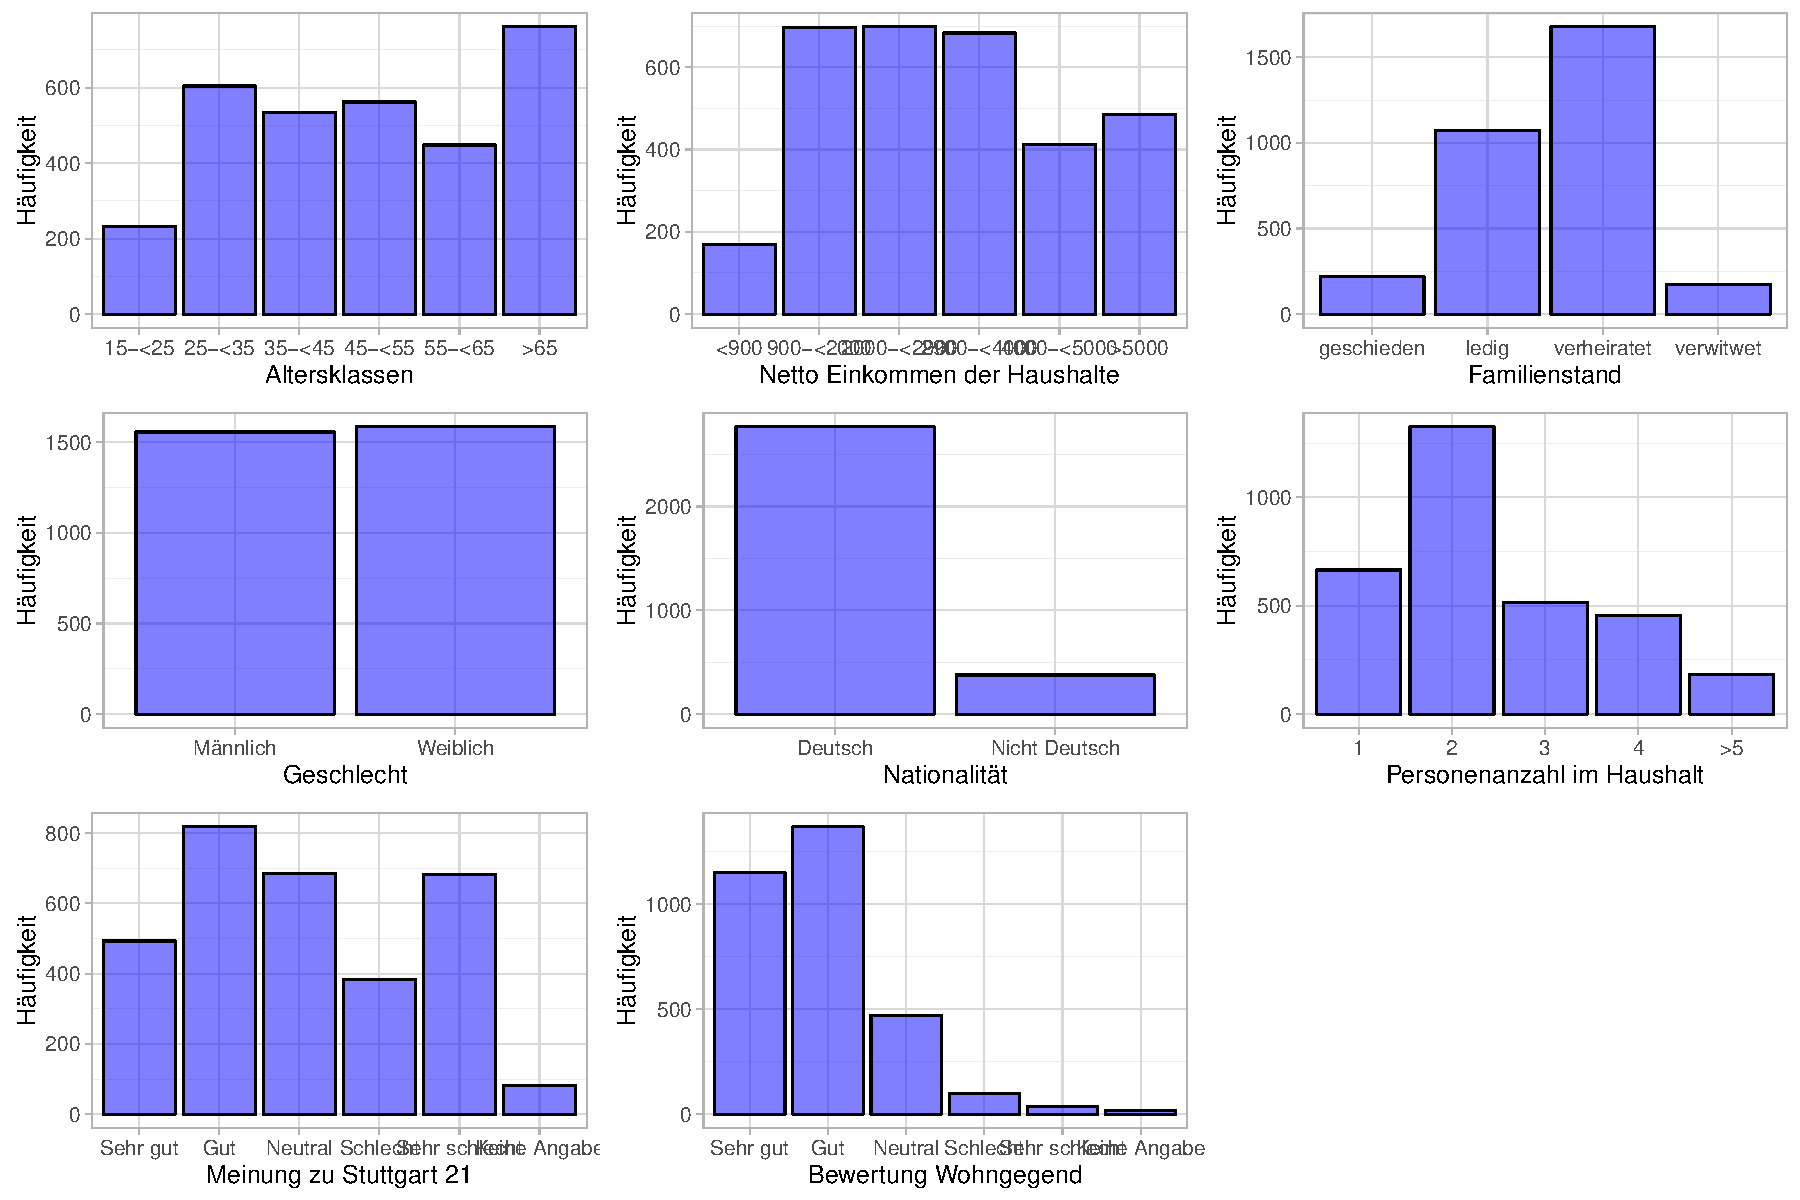
\includegraphics[scale=0.8]{Pictures/BarData}
 \end{center}
\end{figure}

\end{appendix}
\clearpage
\pagestyle{plain}
%\phantomsection
%\addcontentsline{toc}{section}{Eigenständigkeitserklärung}

%\section{Eigenständigkeitserklärung}

Hiermit versichere ich, dass ich die vorliegende Hausarbeit selbstständig verfasst und keine anderen als die angegebenen
Hilfsmittel benutzt habe. Alle wörtlich oder sinngemäß den Schriften anderer entnommenen Stellen
habe ich unter Angabe der Quellen kenntlich gemacht. Dies gilt auch für beigefügte Zeichnungen, Skizzen, bildliche
Darstellungen und dergleichen.\\
\\
Mir ist bewusst, dass ich mich im Falle einer unbeabsichtigten oder vorsätzlichen Missachtung durch den fehlerhaften
Umgang mit Quellen unter Umständen strafbar mache und die vorliegende Hausarbeit mit nicht ausreichend
bewertet wird.
\\
\\Göttingen, den
\\Unteschrift
\vspace*{4cm}
\\
Hiermit erlaube ich, dass meine Arbeit auf Betrug und falsche, sowie fehlende Zitate auch online geprüft wird.\\
\\
Mir ist bewusst, dass ich mich im Falle einer unbeabsichtigten oder vorsätzlichen Missachtung durch den fehlerhaften
Umgang mit Quellen unter Umständen strafbar mache und die vorliegende Hausarbeit mit nicht ausreichend
bewertet wird.
\\
\\Göttingen, den
\\Unterschrift
\clearpage


\end{document}
